88. \begin{figure}[ht!]
\center{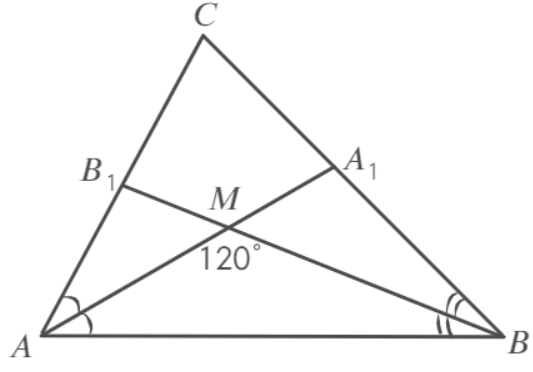
\includegraphics[scale=0.35]{g88.png}}
\end{figure}\\
Обозначим $\angle CAM=\angle MAB=x,\ \angle CBM=\angle MBA=y,$ тогда из треугольника $AMB$ имеем $x+y+120^\circ=180^\circ,\ x+y=60^\circ.$ Тогда из треугольника $ABC:\ 2x+2y+\angle C=180^\circ,\ \angle C=180^\circ-2\cdot60^\circ=60^\circ.$\newpage
\noindent89. \begin{figure}[ht!]
\center{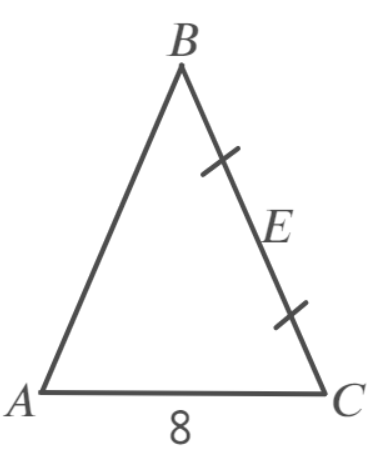
\includegraphics[scale=0.35]{g89.png}}
\end{figure}\\
Одна часть периметра равна $AB+BE,$ а другая --- $EC+8.$ Так как $BE=EC,$ отличаются они на столько же, на сколько отличаются $AB$ и 8. Значит $AB$ может быть равно 6 или 10.\\
